
\chapter{Nuclear Physics in Ultra-relativistic Heavy-Ion Collisions}

\section{The Standard Model}

The Standard Model describes the fundamental particles of the universe in terms of fermions and bosons. Fermions are particles with half-integer spin, while bosons have integer-spin. This difference in spin has far reaching consequences. Fermions must obey the Pauli Exclusion Principle: only one fermion at a time can occupy a given state. However, multiple bosons can simultaneously occupy a specific state.

Among the fermions are the leptons, neutrinos, and quarks. The leptons consist of the electron, muon, and tau, as well as their anti-particles. The leptons are seemingly fundamental: high energy experiments have yet to observe internal lepton-structure. Neutrinos are weakly interacting particles detected primarily through the precise measuring of missing transverse energy in the products of particle collisions. Quarks are the constituent particles of baryons, which contain three valence quarks, and mesons, which contain two valence quarks. In addition to the valence quarks are the sea quarks, which appear and disappear as quark-antiquark pairs within hadrons. The hadrons are particles made of quarks and gluons.

The behavior of fundamental particles is best described within the framework of quantum field theory (QTF). QFT defines a Lagrangian for fundamental particles. This Lagrangian then predicts the outcome of particle collisions. Different terms in the Lagrangian correspond to the various interactions between particles. The Standard Model Lagrangian can be broken down into four basic terms:

\begin{equation}
\mathcal{L}_{Standard Model} = \mathcal{L}_{QED} + \mathcal{L}_{QCD} + \mathcal{L}_{Higgs} + ... 
\end{equation}

The QED and QCD Lagrangians will be the most important in what follows. Feynman rules are derived from the Langrangian. Particularly important for the Feynman rules are the coupling constants for the electromagnetic force and strong-nuclear force.

\subsection{Quantum Electrodynamics}

Quantum electrodynamics (QED) is a theory of electromagnetic interaction in terms of relativistic quantum field theory. QED addresses three specific processes: photon motion, electron motion, and the emission, or absorption, of a photon by an electron.

The QED coupling decreases with distance, as manifest the Coulomb force being proportional to an inverse-square law. 

\begin{equation}
\alpha_{QED}(Q^2) = \frac{ \alpha_{em}}{(1 - \frac{\alpha_{em}}{3\pi})\mathrm{ln}(\frac{Q^2}{m^2}) }
\end{equation}

\subsection{Quantum Chromodynamics}

The quarks are a family of fermions that compose the baryons and the mesons. Baryons consist of three quarks in a color neutral state, while mesons consist two quarks in a color neutral state. "Color" in this context refers to the six kinds of strongly-interacting charge available to quarks: red and anti-red, blue and anti-blue, and green and anti-green. Color charge has no relation to optical phenomena, but provides a useful analogy for the stable combinations of quarks. The net color-charge of a baryon or meson is "white".

Unlike QED, the QCD coupling increases with distance. This has the practical consequence of the strong-interactions being stronger in high momentum transfer collisions. The direct results of the running QCD coupling are the dual phenomena of asymptotic freedom and color confinement. At large distances, string tension describes the binding force of the quarks. At short distances, however, Coulomb-like interactions dominate.

Within the nucleus, a proton can be thought of as a bubble in a vacuum. Debrye screening exerts a pressure on the proton. This pressure is responsible for the size of the proton. 

\begin{equation}
\alpha_{QCD}(Q^2) = \alpha_{s}(Q^2) = \frac{4 \pi }{(11 - \frac{2}{3}n_f)\mathrm{ln}(\frac{Q^2}{\Lambda^2_{QCD}}) }
\end{equation}


\section{QCD Experiments}

Scattering experiments are the basic tool for exploring the nucleus. The Large Hadron Collider (LHC) is capable of reaching heavy-ion collision energies of up to 7 TeV per nucleon-nucleon. The higher the energy, the more experiments can probe the nuclear phase-space diagram.

At the turn of the century, Ernst Rutherford probed the gold atom by bombarding a gold sheet with alpha-particles (helium nuclei). The angular distribution of the scattered alpha-particles demonstrates that the mass of the atom is concentrated in a small volume, i.e, the atom is mostly empty space. 

Momentum transferred, expressed as $Q^2$, is an important quantity for characterizing QCD measurements. 

In addition to $Q^2$, Bjorken-x, also known as Bjorken-scaling is necessary to describe the nuclear phase space. Bjorken-x represents the momentum fraction of partons. 

\subsection{Hard Processes}

Hard processes involve scattering particles off partons in the manner of point-like charges.

\subsubsection{Deep Inelastic Scattering}

Deep inelastic scattering commonly refers to the scattering of a leptons off hadrons. These experiments provided the first evidence of Bjorken-scaling in the nucleus, a direct interpretation of which is the existence of quarks as point-like particles at high energies.

\subsection{Soft Processes}
Soft processes compose the low momentum transfer, typically gluon-gluon interactions during a  collision.

\subsection{Heavy-Ion Collisions}

Similar to the Rutherford experiment, in heavy-ion collisions the scattered particles carry information about the internal structure of the nucleus. 

The Rutherford experiment has the three components that still characterize high-energy nuclear experiments: a probe, a medium, and a signal. Alpha particles probe the medium of the gold atom, and the angular distribution of scattered alpha particles signals the internal structure of the atom. 

\subsubsection{Ultra-peripheral Collisions}

Ultra-peripheral collisions occur at impact parameters greater than the sum of the heavy-ion radii. In these collisions, hadronic interactions are strongly suppressed while photonuclear activity is enhanced proportional to the square of the nuclear charge. The electromagnetic field of an incoming heavy-ion, from the perspective of a target, is equivalent to a flux of virtual photons. 

\section{Jet Production}

Gluons are the particle exchanged in strong interactions. However, gluons themselves carry color charge. By analogy, photons transmit the electromagnetic force, but do not themselves have an electric charge. 

When a quark is scattered from a nucleus, the strong interaction gathers potential energy until the threshold for quark production is passed, at which point an anti-quark is generated to screen the ejected quark.

\subsection{Diffraction}

QCD factorisation describes the diffractive-photoproduction dijet cross-section as the convolution of the partonic cross-section with the diffractive parton distributions. However, factorisation only describes H1 data if the resolved-photon contribution is suppressed. 

\subsection{Photoproduction}

The photoproduction cross-section is proportional to the gluon distribution.

\centerline{
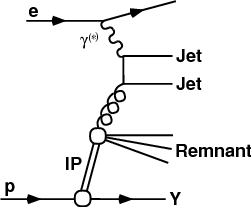
\includegraphics[width=2in]{Chapter1/importfigs/fig1a.png}
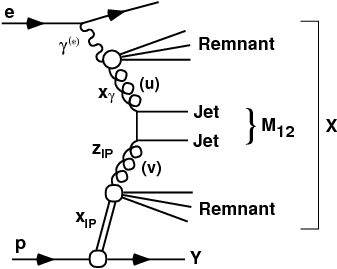
\includegraphics[width=2in]{Chapter1/importfigs/fig1b.png}
}

\subsubsection{Direct Photon Processes}

At low momentum transfer, photons interact electromagnetically, i.e. directly, with partons. 

\subsubsection{Resolved Photon Processes}

High energy photons possess a hadronic structure. 